



\begin{section}{Ejercicio 6}
Realizar un grafico de los ECM con b = 1 y n = 15, 30, 50, 100, 150, 200 ¿Que observa? ¿Que
estimador elige? ¿Que sospecha sobre la consistencia de los estimadores?

\begin{subsection}{Implementacion}


Se utiliza el siguiente codigo para generar los vectores.
\begin{verbatim}
b = 1;
ni = double();
ni <- c(15, 30, 50, 100, 150, 200);
niLen = 6;
momSims = double();
medSims = double();
mvSims = double();

for(i in 1:niLen){
	momSims[i] <- simulacion_mom(b,ni[i]);
	medSims[i] <- simulacion_med(b,ni[i]);
	mvSims[i] <- simulacion_mv(b,ni[i]);
}

\end{verbatim}

Y luego creamos los graficos compuestos con sl siguiente codigo:

\begin{verbatim}

> plot(ni, momSims, ylim=c(0,0.030))
> points(ni, medSims , col="red")
> points(ni, mvSims , col="green")
> 

\end{verbatim}

Se obtiene el siguiente grafico, donde los puntos de color negro son los de $B_{mom}$, los de color rojo los de $B_{med}$, y los de color verde los de $B_{mv}$.


Error cuadratico medio de $B_{mom}$
\begin{figure}[H]
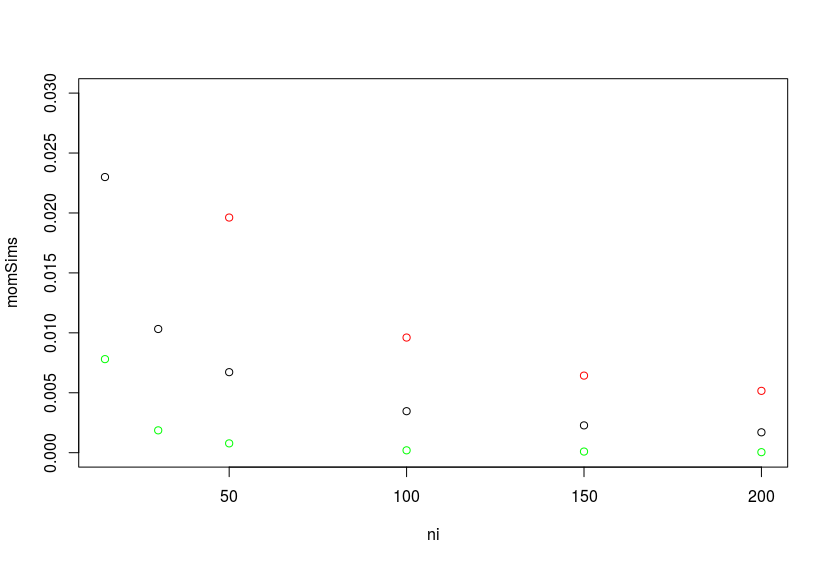
\includegraphics[scale=0.65]{plots/combNPlot.png}
\centering
\end{figure}
~\\
~\\



Nuevamente se observa una convergencia mas rapida para el estimador de maxima verosimilitud. Ademas, en cuanto a la consistencia, el unico estimador que converge al valor real, al menos con $n<200$, es el de maxima verosimilitud, con lo cual es el unico que parece consistente.
\end{subsection}
\end{section}